\documentclass{report}          % Definimos el tipo de documento

%% Paquetes
    % Paquetes de Formato y Tipografía
        \usepackage[T1]{fontenc}            % Codificación de fuente que mejora la salida en PDF
        \usepackage[utf8]{inputenc}         % Permite el uso de caracteres especiales (tildes, ñ, etc.)
        \usepackage[letterpaper,top=2cm,bottom=2cm,left=2.5cm,right=2.5cm]{geometry}
        \usepackage{lmodern}                 % Especificamos la fuente
        \hyphenation{co-mer-cial rea-li-zan si-guien-te si-mu-la-ción ke-lly con-si-de-ra-da}                   % Silabeo de palabras


    % Paquetes de Idioma
        \usepackage[spanish]{babel}         % Configura el idioma a español (traduce títulos, orden de palabras, etc.)
        \spanishdecimal{.}                  % Establece el punto como separador decimal en español

    % Paquetes Matemáticos
        \usepackage{amsmath}      % Soporte para ecuaciones matemáticas avanzadas
        \usepackage{amssymb}      % Símbolos matemáticos adicionales
        \usepackage{mathrsfs}     % Fuente matemática caligráfica

    % Paquetes para Figuras y Tablas
        \usepackage{graphicx}      % Permite incluir imágenes en el documento
        \usepackage{float}         % Controla la posición de imágenes y tablas
        \usepackage{subfigure}     % Permite incluir subfiguras dentro de una figura
        \usepackage{tabularx}      % Mejora el control de tablas con ancho ajustable
        \usepackage[table]{xcolor} % Permite usar colores en tablas

    % Paquetes de Hipervínculos y Referencias
        \usepackage{natbib}                           % Manejo de referencias bibliográficas
        \usepackage[colorlinks=true, allcolors=blue]{hyperref} % Habilita enlaces internos y externos en color azul
        \bibpunct{(}{)}{;}{a}{,}{,}                  % Configuración del formato de citas

    % Paquetes para formato de Código Fuente
        \usepackage{listingsutf8}     % Paquete para mostrar código fuente con sintaxis destacada
        \definecolor{codegreen}{rgb}{0,0.6,0}  % Color para comentarios en código
        \definecolor{codegray}{rgb}{0.5,0.5,0.5} % Color para números de línea
        \definecolor{codepurple}{rgb}{0.58,0,0.82} % Color para cadenas de texto
        \definecolor{backcolour}{rgb}{0.95,0.95,0.92} % Color de fondo para bloques de código

        \lstdefinestyle{mystyle} 
        {
            frame=single,                       % Marco alrededor del código
            backgroundcolor=\color{white},      % Fondo blanco
            commentstyle=\color{codegreen},     % Comentarios en verde
            keywordstyle=\color{magenta},       % Palabras clave en magenta
            numberstyle=\tiny\color{codegray},  % Números de línea en gris
            stringstyle=\color{codepurple},     % Cadenas en púrpura
            basicstyle=\ttfamily\footnotesize,  % Fuente monoespaciada pequeña
            breaklines=true,                    % Permitir saltos de línea en código
            captionpos=b,                       % Coloca los títulos del código abajo
            numbers=left,                       % Números de línea a la izquierda
            tabsize=2                           % Espaciado de tabulación de 2
        }
        \lstset{style=mystyle}                  % Aplica el estilo definido
        \lstset{inputencoding=utf8/latin1}      % Permite caracteres especiales en código

    % Paquetes para Diagramas y Gráficos
        \usepackage{tikz}                           % Paquete para gráficos vectoriales
        \usetikzlibrary{shapes.geometric, arrows}   % Librerías de TikZ para diagramas de flujo

    % Definición de estilos de nodos y flechas en diagramas de flujo
        \tikzstyle{process} = [rectangle, minimum width=3cm, minimum height=1cm, text centered, draw=black]
        \tikzstyle{arrow} = [thick,->,>=stealth]

% Macros para palabras importantes
    \newcommand{\fullname}      {Sistema Automatizado de Corrección y Monitoreo Energético (SACME)}
    \newcommand{\shortname}     {SACME}
    \newcommand{\docdate}       {15 de marzo del 2025}

%---------------------------------------------------------------------%

\begin{document}

    %----------------- PORTADA -----------------%
    \begin{titlepage}
        \centering
        \begin{figure}[ht]
            \centering
            
\includegraphics[width=0.3\textwidth]{Recursos/Imagenes/Portada/logos_fi_uaq.png}
        \end{figure}
        
        \vspace{1cm}
        {\scshape\LARGE Universidad Autónoma de Querétaro \par}
        \vspace{0.5cm}
        {\scshape\Large Facultad de Ingeniería \par}
        \vspace{0.5cm}
        {\scshape\Large Ingeniería en Automatización \par}
        
        \vspace{1.5cm}
        {\Large\bfseries T.D.T.A. IV \par}
        
        \vspace{1cm}
        {\Large\bfseries \fullname \par}
        
        \vspace{1.5cm}
        {\large \textbf{Profesor:} \par}
        {\large Dr. Gonzalo Macías Bobadilla \par}
        
        \vspace{1.5cm}
        {\large \textbf{Integrantes:} \par}
        \begin{center}
            \large
            Zúñiga Fragoso Diego Joel\par
            \vspace{0.4cm}
            Manríquez Navarro Daniela del Carmen\par
            \vspace{0.4cm}
            Zeron Marin Luis Alejandro\par
            \vspace{0.4cm}
            González Caballero Luis Fernando\par
        \end{center}
        
        \vfill      % Rellenamos espacio restante

        {\large Fecha de entrega: \docdate \par}
    \end{titlepage}

    \clearpage  % Salto de página sin numeración

    \tableofcontents        % Índice en números romanos
    \thispagestyle{empty} % Elimina la numeración en la página del índice
    \listoffigures             % Lista de figuras
    \thispagestyle{empty} % Elimina la numeración en la página del índice
    \listoftables              % Lista de tablas
    \thispagestyle{empty} % Elimina la numeración en la página del índice
    \newpage

    \pagenumbering{arabic}  % Cambio a números arábigos en el contenido principal
    \setcounter{page}{1}   % Asegura que comience desde "1"
    %----------------- RESUMEN -----------------%
    \chapter{Resumen}
        Este proyecto desarrolla un \fullname, diseñado para optimizar el consumo eléctrico en instalaciones industriales y comerciales. El sistema corrige el factor de potencia en tiempo real mediante la conexión y desconexión automática de bancos de capacitores, evitando penalizaciones por bajo factor de potencia y reduciendo las pérdidas de energía. Además, integra un módulo de monitoreo remoto basado en IoT (Internet de las Cosas), que permite visualizar los parámetros eléctricos a través de una plataforma web o aplicación móvil. \par
        El dispositivo utiliza sensores y medidores robustos para capturar datos en tiempo real, como voltaje, corriente, potencia activa, reactiva y factor de potencia. Estos datos son procesados por un controlador central que activa los bancos de capacitores según la demanda reactiva. La conectividad IoT permite el envío de datos a un servidor en la nube, donde se generan reportes y alertas para el usuario, facilitando la identificación de anomalías y la toma de decisiones informadas.

    %----------------- INTRODUCCION -----------------%
    \chapter{Introducción}
        El factor de potencia es un parámetro clave en la eficiencia energética de cualquier instalación eléctrica. Un bajo factor de potencia genera pérdidas económicas y problemas en la red. En este trabajo se desarrolla un banco de capacitores automático capaz de corregir el factor de potencia en tiempo real y permitir su monitoreo remoto mediante IoT.
        
        \section{Planteamiento del problema}

        \section{Objetivos generales}

        \section{Objetivos específicos}


    %----------------- FUNDAMENTACION TEORICA -----------------%
    \chapter{Fundamentación teórica}  
        La monitorización y optimización de la potencia eléctrica son procesos fundamentales para garantizar la eficiencia energética en instalaciones industriales y comerciales. Para lograr una gestión efectiva de la energía, es necesario comprender los factores que afectan negativamente su consumo, así como las tecnologías y metodologías disponibles para mitigar estos efectos. Este marco teórico tiene como objetivo proporcionar los fundamentos conceptuales y técnicos que sustentan el desarrollo del \shortname, enfocándose en la corrección del factor de potencia y la monitorización en tiempo real de parámetros eléctricos.
    
        \section{Potencia eléctrica}
            La potencia eléctrica es la tasa a la que se transfiere o se transforma energía en un sistema eléctrico. Se mide en vatios (W) y es fundamental para determinar la capacidad de un circuito o dispositivo para realizar trabajo, ya sea en forma de calor, movimiento o luz.\\
            En términos generales, la potencia eléctrica indica cuánta energía se consume o se genera por unidad de tiempo.
            
            \subsection{Potencia eléctrica en circuitos de corriente directa (DC)}
            En un circuito de corriente continua (DC), la potencia eléctrica es directamente proporcional al voltaje aplicado y a la corriente que fluye a través del circuito. Dado que en estos circuitos la impedancia está compuesta únicamente por elementos resistivos, la ecuación que describe la potencia es sencilla y se expresa de la siguiente manera:

            \begin{equation}
                P=V*I
            \end{equation}
            Donde:
            \begin{itemize}
                \item $P$: Es la potencia eléctrica en watts [W]
                \item $V$: Es la tension o voltaje en voltios [V]
                \item $I$: Es la corriente eléctrica en amperios [A]
            \end{itemize}

            \subsection{Triangulo de potencia}
            El Triángulo de Potencia es una representación gráfica que permite visualizar y relacionar las tres magnitudes fundamentales en un sistema de corriente alterna: la potencia activa, la potencia reactiva y la potencia aparente. Este diagrama facilita el análisis del comportamiento del sistema y la eficiencia en el uso de la energía.\par

            \begin{figure}[H]
                \label{fig:DiagramaEje}
                \centering
                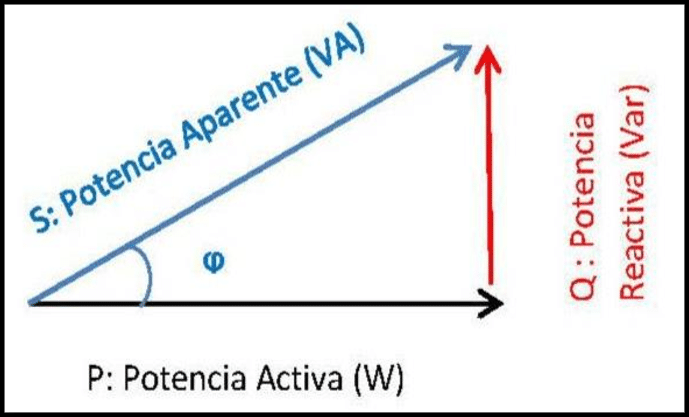
\includegraphics[width=0.4\textwidth] {Recursos/Imagenes/Marco_teorico/Triangulo_de_potencia.png}
                \caption{Imagen ilustrativa del triangulo de potencia}
            \end{figure}

            Donde:
            \begin{itemize}
                \item Potencia Activa (P): \par
                    Representa la energía que efectivamente se convierte en trabajo útil (calor, movimiento, luz, etc.) y se mide en vatios [W]. Se ubica en el eje horizontal.
                \item Potencia Reactiva (Q):\par
                    Es la energía que oscila entre la fuente y la carga, debida a los elementos inductivos y capacitivos, y se mide en voltamperios reactivos [VAR]. Se ubica en el eje vertical.
                \item Potencia Aparente (S): \par
                    Es el vector resultante que combina la potencia activa y reactiva, y se mide en voltamperios [VA]. Es la hipotenusa del triángulo.
            \end{itemize}

            Debido a la existencia de la potencia reactiva en circuitos de corriente alterna, no toda la potencia se convierte en trabajo debido al desfase entre el voltaje y la corriente. Por lo tanto, la fórmula de la potencia quedara expresada de la siguiente manera:

            \begin{equation}
                P=V*I*cos(\phi)
            \end{equation}
            Donde:
            \begin{itemize}
                \item $cos(\phi)$: Es el factor de potencia
            \end{itemize}
        
        \section{Definicion e impacto del factor de potencia}
            El factor de potencia (FP) es un indicador que mide la eficiencia con la que se utiliza la energía eléctrica. Matemáticamente, se define como la relación entre la potencia activa (P) y la potencia aparente (S), y coincide con el coseno del ángulo de desfase ($\phi$) entre la tensión y la corriente.

            \begin{equation}
                FP = \frac{P}{S} = \cos(\phi)
            \end{equation}

            El factor de potencia puede tomar valores entre 0 y 1, donde:
            \begin{itemize}
                \item FP = 1: Indica un circuito puramente resistivo donde toda la energía consumida se convierte en trabajo útil.
                \item FP = 0: Representa un circuito puramente inductivo o capacitivo donde toda la energía oscila entre la fuente y la carga sin producir trabajo útil.
            \end{itemize}
        
            En instalaciones industriales, un factor de potencia óptimo se considera por encima de 0.95. La Comisión Federal de Electricidad (CFE) en México establece penalizaciones económicas para consumidores con un factor de potencia inferior a 0.9, mientras que ofrece bonificaciones para aquellos que mantienen valores superiores a este umbral.

            \subsection{Elementos que afectan al factor de potencia}
                Diversos elementos presentes en las instalaciones eléctricas pueden reducir el factor de potencia debido a su comportamiento inductivo o capacitivo. Los más comunes son:
    
                \begin{itemize}
                    \item \textbf{Motores eléctricos de inducción}: Representan la carga inductiva más significativa en la industria. Consumen potencia reactiva para generar sus campos magnéticos, especialmente cuando operan por debajo de su capacidad nominal.
                    
                    \item \textbf{Transformadores}: Requieren potencia reactiva para la magnetización de sus núcleos. Cuando operan con baja carga, el consumo de potencia reactiva puede ser proporcionalmente alto.
                    
                    \item \textbf{Equipos de iluminación con balastros electromagnéticos}: Particularmente las lámparas fluorescentes y de descarga de alta intensidad tradicionales que utilizan balastros inductivos.
                    
                    \item \textbf{Máquinas de soldar}: Los equipos de soldadura por arco eléctrico tienen un factor de potencia inherentemente bajo debido a su alta inductancia.
                    
                    \item \textbf{Hornos de inducción}: Utilizan campos electromagnéticos para calentar materiales, lo que genera un consumo elevado de potencia reactiva.
                    
                    \item \textbf{Equipos electrónicos con fuentes conmutadas}: Aunque individualmente pueden tener un impacto menor, su proliferación en entornos industriales y comerciales suma un efecto considerable.
                \end{itemize}

            \subsection{Consecuencias de un bajo factor de potencia}
                Un factor de potencia deficiente tiene implicaciones técnicas y económicas significativas:
    
                \begin{itemize}
                    \item \textbf{Penalizaciones económicas}: Las empresas suministradoras de energía aplican recargos en la facturación cuando el factor de potencia está por debajo de ciertos límites (típicamente 0.9), pudiendo incrementar el costo de la energía hasta en un 20\%.
                    
                    \item \textbf{Sobrecarga en conductores}: La corriente total que circula aumenta inversamente proporcional al factor de potencia, causando mayores pérdidas por efecto Joule ($I^2R$) y exigiendo conductores de mayor sección.
                    
                    \item \textbf{Sobrecarga en transformadores}: Reduce la capacidad efectiva de los transformadores para suministrar potencia activa, ya que parte de su capacidad se destina a la potencia reactiva.
                    
                    \item \textbf{Caídas de tensión}: El incremento de corriente provoca mayores caídas de tensión en la línea, afectando la calidad del suministro y el funcionamiento de equipos sensibles.
                    
                    \item \textbf{Reducción de la capacidad del sistema eléctrico}: Limita la cantidad de carga útil que puede conectarse a la red existente, pudiendo requerir ampliaciones innecesarias de la instalación.
                    
                    \item \textbf{Mayor desgaste en equipos de distribución}: Interruptores, seccionadores y protecciones sufren mayor estrés debido a las corrientes elevadas.
                \end{itemize}
        
                En términos cuantitativos, cuando el factor de potencia disminuye de 0.95 a 0.75, la capacidad del sistema se reduce aproximadamente en un 21\%, mientras que las pérdidas en conductores aumentan en un 60\%.

        \section{Corrección del factor de potencia}
            La corrección del factor de potencia consiste en la instalación de dispositivos que compensen la potencia reactiva consumida por las cargas inductivas. El objetivo es acercar el factor de potencia lo más posible a la unidad, minimizando así la potencia reactiva que debe suministrar la red eléctrica.
            
            El método más común de corrección es la instalación de capacitores, que proporcionan potencia reactiva de carácter opuesto a la consumida por las cargas inductivas. La capacidad necesaria para la corrección se puede calcular mediante la siguiente fórmula:
            
            \begin{equation}
                Q_c = P \times (\tan\phi_1 - \tan\phi_2)
            \end{equation}
            
            Donde:
            \begin{itemize}
                \item $Q_c$: Potencia reactiva capacitiva necesaria en VAR
                \item $P$: Potencia activa consumida en W
                \item $\phi_1$: Ángulo del factor de potencia inicial
                \item $\phi_2$: Ángulo del factor de potencia deseado
            \end{itemize}
    
            \subsection{Métodos actuales de corrección del factor de potencia}
                Existen diferentes enfoques para implementar la corrección del factor de potencia, cada uno con sus propias ventajas y aplicaciones:
    
                \begin{itemize}
                    \item \textbf{Corrección individual}: Consiste en instalar capacitores directamente en los bornes de cada equipo con bajo factor de potencia. Presenta ventajas como la descarga de los conductores desde la fuente hasta la carga y la automatización intrínseca (los capacitores operan solo cuando el equipo está en funcionamiento). Es ideal para motores y equipos de gran potencia con ciclos prolongados de operación.
                    
                    \item \textbf{Corrección por grupos}: Se aplica cuando un conjunto de cargas opera simultáneamente. Los capacitores se instalan en un punto común que alimenta a todo el grupo, como un tablero de distribución secundario. Ofrece un equilibrio entre costo y eficiencia, reduciendo el número de capacitores necesarios.
                    
                    \item \textbf{Corrección centralizada}: Un banco de capacitores se instala en el punto principal de alimentación, generalmente junto al transformador o en el tablero general. Este método requiere un sistema de control automático para ajustar la capacitancia según la demanda variable de potencia reactiva.
                    
                    \item \textbf{Bancos automáticos de capacitores}: Utilizan controladores electrónicos que monitorean continuamente el factor de potencia y conectan o desconectan escalones de capacitores según sea necesario. Estos sistemas incluyen:
                    \begin{itemize}
                        \item Sensores de voltaje y corriente
                        \item Relés varimétricos que detectan cambios en la potencia reactiva
                        \item Controladores microprocesados que determinan qué pasos de capacitores activar
                        \item Contactores para la conexión/desconexión física de los capacitores
                        \item Resistencias de descarga para proteger los capacitores durante la conmutación
                    \end{itemize}
                    
                    \item \textbf{Filtros activos}: Dispositivos electrónicos de potencia que generan corrientes armónicas de igual magnitud pero fase opuesta a las generadas por las cargas no lineales. Además de corregir el factor de potencia, estos sistemas mejoran la calidad de la energía eliminando armónicos. Son especialmente útiles en instalaciones con alta presencia de equipos electrónicos y variadores de frecuencia.
                    
                    \item \textbf{Compensadores síncronos}: Motores síncronos que funcionan en vacío, pudiendo generar o absorber potencia reactiva mediante el ajuste de su excitación. Aunque presentan ventajas en aplicaciones de gran escala, su uso ha disminuido debido a su alto costo y mantenimiento frente a soluciones más modernas.
                \end{itemize}

                La elección del método más adecuado depende de varios factores, incluyendo el tipo de carga, el patrón de consumo, la estabilidad de la demanda y las consideraciones económicas. En instalaciones industriales modernas, la tendencia es hacia sistemas automatizados con monitoreo en tiempo real que permitan una respuesta dinámica a las variaciones de carga y optimicen el consumo energético global.
        
    %----------------- METODOLOGIA -----------------%
    \chapter{Metodología}
        Para el desarrollo del \shortname, se implementó una metodología estructurada basada en el diseño de sistemas embebidos, integrando consideraciones específicas para aplicaciones industriales de potencia y conectividad IoT. El proceso se dividió en varias etapas interrelacionadas que permitieron avanzar desde la concepción teórica hasta la implementación y validación del sistema final.
        \section{Especificación}
            El primer paso consistió en definir las especificaciones técnicas y funcionales que debía cumplir el sistema, basadas en los requerimientos de instalaciones industriales típicas y las limitaciones identificadas en soluciones existentes.
        
            \subsection{Requerimientos funcionales}
                Se establecieron los siguientes requerimientos funcionales esenciales:
        
                \begin{itemize}
                    \item \textbf{Corrección automática del factor de potencia}: El sistema debe mantener un factor de potencia superior a 0.95 bajo condiciones variables de carga, mediante la conexión y desconexión controlada de bancos de capacitores.
                    
                    \item \textbf{Medición precisa de parámetros eléctricos}: Capacidad para medir voltaje, corriente, potencia activa, potencia reactiva, factor de potencia y componentes armónicos con precisión de clase 0.5 o superior según IEC 62053-22.
                    
                    \item \textbf{Monitoreo remoto}: Transmisión segura de datos a una plataforma en la nube, con accesibilidad mediante interfaz web y aplicación móvil.
                    
                    \item \textbf{Alertas y notificaciones}: Generación automática de alertas ante condiciones anómalas, como factor de potencia por debajo del umbral establecido, sobrecalentamiento de capacitores o fallos en el sistema.
                    
                    \item \textbf{Registro histórico}: Almacenamiento y visualización de datos históricos para análisis de tendencias y generación de informes.
                    
                    \item \textbf{Operación autónoma}: Funcionamiento continuo sin intervención manual, con capacidad de autodiagnóstico y recuperación ante fallos.
                \end{itemize}
            
            \subsection{Especificaciones técnicas}
                Con base en los requerimientos funcionales, se establecieron las siguientes especificaciones técnicas:
        
                \begin{itemize}
                    \item \textbf{Tensión nominal}: Sistema trifásico 220/440 VAC, compatible con configuraciones delta y estrella.
                    
                    \item \textbf{Capacidad de corrección}: Hasta 100 kVAR, distribuidos en módulos de 5 kVAR para permitir una corrección escalonada.
                    
                    \item \textbf{Resolución de medición}: 
                    \begin{itemize}
                        \item Voltaje: ±0.5\% en rango 80-500 VAC
                        \item Corriente: ±0.5\% en rango 1-1000 A (mediante transformadores de corriente)
                        \item Factor de potencia: ±0.01
                        \item Armónicos: Hasta el 25º orden con precisión de ±2\%
                    \end{itemize}
                    
                    \item \textbf{Frecuencia de muestreo}: 12.8 kHz para análisis de calidad de energía (256 muestras por ciclo en red de 50 Hz).
                    
                    \item \textbf{Tiempo de respuesta}: Menos de 5 segundos para cambios significativos en la demanda de potencia reactiva.
                    
                    \item \textbf{Conectividad}: Ethernet industrial (Modbus TCP/IP), Wi-Fi (802.11b/g/n) y comunicación celular 4G como respaldo.
                    
                    \item \textbf{Condiciones ambientales}: Operación en entornos industriales con temperatura ambiente -10°C a 60°C y humedad relativa hasta 95\% sin condensación.
                    
                    \item \textbf{Normativas aplicables}: Cumplimiento con normas IEC 61000-4 (EMC), IEC 60831 (capacitores de potencia), IEC 61010 (seguridad) y UL 508A (paneles de control industrial).
                \end{itemize}
            
        \section{Diseño}
            La fase de diseño se dividió en tres subsistemas interconectados: adquisición de datos, procesamiento y control, y conectividad IoT. Para cada uno se evaluaron distintas alternativas tecnológicas, seleccionando finalmente la arquitectura más adecuada para cumplir con los requerimientos establecidos.
        
            \subsection{Evaluación de plataformas de procesamiento}
                Se realizó un análisis comparativo entre plataformas ESP32 y FPGA, considerando aspectos críticos para la aplicación:
        
                \begin{table}[H]
                    \centering
                    \begin{tabular}{|p{3cm}|p{5cm}|p{5cm}|}
                        \hline
                        \textbf{Criterio} & \textbf{ESP32} & \textbf{FPGA} \\
                        \hline
                        Capacidad de procesamiento & Dual-core hasta 240 MHz, suficiente para cálculos básicos de potencia & Superior, permite procesamiento paralelo para análisis avanzado en tiempo real \\
                        \hline
                        Velocidad de muestreo & Limitada por ADC (hasta 500 ksps) & Superior, permitiendo muestreo simultáneo de múltiples canales a alta frecuencia \\
                        \hline
                        Conectividad integrada & Wi-Fi y Bluetooth incorporados & Requiere componentes adicionales \\
                        \hline
                        Complejidad de desarrollo & Programación en C/C++, amplia disponibilidad de bibliotecas & Mayor complejidad, lenguajes HDL (VHDL/Verilog) \\
                        \hline
                        Costo & Bajo (5-15 USD) & Moderado a alto (50-300 USD) \\
                        \hline
                        Escalabilidad & Limitada por recursos de hardware & Alta, configurable según necesidades \\
                        \hline
                        Consumo energético & Bajo, modos de ahorro de energía & Variable, típicamente mayor \\
                        \hline
                        Robustez industrial & Limitada, requiere acondicionamiento & Mayor tolerancia a entornos industriales \\
                        \hline
                    \end{tabular}
                    \caption{Comparativa entre plataformas ESP32 y FPGA}
                \end{table}
        
                Tras evaluar las ventajas y limitaciones de cada plataforma, se optó por una arquitectura híbrida que combina:
        
                \begin{itemize}
                    \item \textbf{FPGA Xilinx Artix-7} como núcleo de procesamiento para la adquisición de datos y cálculos de parámetros eléctricos en tiempo real, aprovechando su capacidad de procesamiento paralelo y alta velocidad de muestreo.
                    
                    \item \textbf{Microcontrolador ARM Cortex-M4F} para la implementación de algoritmos de control, gestión de interfaces de usuario locales y coordinación general del sistema.
                    
                    \item \textbf{Módulo ESP32} dedicado a la conectividad IoT, permitiendo la comunicación inalámbrica con la plataforma en la nube, con capacidad de actualización remota de firmware.
                \end{itemize}
                
                Esta arquitectura permitió optimizar el balance entre rendimiento, flexibilidad y costo, asegurando el cumplimiento de los requerimientos técnicos establecidos para el sistema.
            
            \subsection{Diseño del subsistema de adquisición de datos}
                El subsistema de adquisición se diseñó para capturar con precisión los parámetros eléctricos fundamentales para el cálculo del factor de potencia y la calidad de energía. Se optó por una arquitectura modular que incluye:
                
                \begin{figure}[H]
                    \centering
                    % Aquí iría el diagrama del subsistema de adquisición de datos
                    % \includegraphics[width=0.8\textwidth]{Imagenes/diagrama_adquisicion.pdf}
                    \caption{Arquitectura del subsistema de adquisición de datos}
                \end{figure}
            
                \begin{itemize}
                    \item \textbf{Acondicionamiento de señales}: 
                    \begin{itemize}
                        \item Transformadores de voltaje con aislamiento galvánico 4 kV para muestreo de voltaje de línea.
                        \item Transformadores de corriente de núcleo dividido (split-core) con relación configurable hasta 1000:5A.
                        \item Circuitos de protección contra sobretensiones y filtros antialiasing.
                    \end{itemize}
                    
                    \item \textbf{Conversión analógica-digital}: 
                    \begin{itemize}
                        \item Convertidores ADC simultáneos de 16 bits, 1 MSPS (ADS8688) para voltajes y corrientes.
                        \item Sincronización de muestreo mediante PLL para mantener precisión de fase entre señales.
                    \end{itemize}
                    
                    \item \textbf{Procesamiento de señales en FPGA}:
                    \begin{itemize}
                        \item Implementación de algoritmos DFT (Discrete Fourier Transform) para análisis de componentes armónicos.
                        \item Cálculo en tiempo real de valores RMS, potencia activa, reactiva y aparente mediante bloques DSP dedicados.
                        \item Detección de eventos transitorios mediante análisis wavelet.
                    \end{itemize}
                \end{itemize}

            \subsection{Diseño del subsistema de control}
                El subsistema de control se diseñó para implementar los algoritmos adaptativos que determinan la conexión óptima de escalones de capacitores según las condiciones detectadas. La arquitectura incluye:
                
                \begin{figure}[H]
                    \centering
                    % Aquí iría el diagrama del subsistema de control
                    % \includegraphics[width=0.8\textwidth]{Imagenes/diagrama_control.pdf}
                    \caption{Arquitectura del subsistema de control}
                \end{figure}

                \begin{itemize}
                    \item \textbf{Algoritmo principal de corrección}: Implementación de un controlador PID adaptativo que determina la potencia reactiva capacitiva necesaria para mantener el factor de potencia objetivo, considerando:
                    \begin{itemize}
                        \item Filtrado digital de las variaciones rápidas para evitar oscilaciones.
                        \item Predicción de tendencias mediante modelos ARX (AutoRegressive with eXogenous inputs).
                        \item Compensación de armónicos para evitar resonancias entre capacitores y la inductancia de la red.
                    \end{itemize}
                    
                    \item \textbf{Etapa de potencia para conexión de capacitores}:
                    \begin{itemize}
                        \item Tiristores en configuración back-to-back para conmutación suave en el cruce por cero.
                        \item Circuitos de amortiguamiento (snubber) para reducir transitorios de conmutación.
                        \item Resistencias de descarga para evitar reconexión con capacitores cargados.
                        \item Sensores de temperatura en cada banco para protección térmica.
                    \end{itemize}
                    
                    \item \textbf{Capacitores de potencia}:
                    \begin{itemize}
                        \item Capacitores trifásicos auto-regenerativos con dieléctrico de polipropileno metalizado.
                        \item Especificación para soportar 1.5 veces la corriente nominal debido a armónicos.
                        \item Fusibles individuales para protección contra cortocircuitos.
                        \item Disposición modular para facilitar mantenimiento y expansión.
                    \end{itemize}
                \end{itemize}

            \subsection{Diseño del subsistema de conectividad IoT}
                La arquitectura IoT se diseñó siguiendo un modelo de capas que asegura la transmisión confiable de datos desde el dispositivo hasta el usuario final:

                \begin{figure}[H]
                    \centering
                    % Aquí iría el diagrama de la arquitectura IoT
                    % \includegraphics[width=0.8\textwidth]{Imagenes/arquitectura_iot.pdf}
                    \caption{Arquitectura de la solución IoT para el \shortname}
                \end{figure}
                
                \begin{itemize}
                    \item \textbf{Capa de dispositivo}:
                    \begin{itemize}
                        \item Módulo ESP32-WROOM-32 con antena externa para mejor conectividad.
                        \item Módulo 4G (SIM7600E) como respaldo para entornos sin Wi-Fi disponible.
                        \item Interfaz RS-485 con aislamiento para integración con sistemas SCADA existentes.
                    \end{itemize}
                    
                    \item \textbf{Capa de comunicación}:
                    \begin{itemize}
                        \item Protocolo MQTT con TLS 1.2 para comunicación segura y eficiente.
                        \item Implementación de mecanismos store-and-forward para operación confiable con conectividad intermitente.
                        \item Compresión de datos para optimizar ancho de banda.
                    \end{itemize}
                    
                    \item \textbf{Capa de plataforma}:
                    \begin{itemize}
                        \item Backend basado en arquitectura serverless (AWS Lambda).
                        \item Base de datos de series temporales (InfluxDB) para almacenamiento eficiente de datos históricos.
                        \item Implementación de APIs RESTful para integración con sistemas externos.
                    \end{itemize}
                    
                    \item \textbf{Capa de aplicación}:
                    \begin{itemize}
                        \item Aplicación web responsiva desarrollada en React.js.
                        \item Aplicación móvil nativa para Android e iOS.
                        \item Dashboards interactivos con Grafana para visualización avanzada de datos.
                    \end{itemize}
                \end{itemize}

        \section{Implementación}
            La fase de implementación se dividió en desarrollo de hardware, firmware y software, seguida de la integración de los componentes en un prototipo funcional.
        
            \subsection{Desarrollo de hardware}
                Se diseñaron y fabricaron las siguientes PCBs (Printed Circuit Boards):

                \begin{itemize}
                    \item \textbf{Placa principal de adquisición y procesamiento}:
                        \begin{itemize}
                            \item FPGA Xilinx Artix-7 (XC7A35T) con 33,280 celdas lógicas.
                            \item Microcontrolador STM32F407 (ARM Cortex-M4F a 168 MHz).
                            \item 8 canales de entrada analógica aislados (4 voltajes, 4 corrientes).
                            \item Memoria SDRAM de 64 MB para almacenamiento temporal de formas de onda.
                            \item Memoria Flash de 32 MB para almacenamiento de firmware y configuraciones.
                        \end{itemize}

                    \item \textbf{Placa de interfaz de potencia}:
                        \begin{itemize}
                            \item Módulos de drivers para tiristores con aislamiento óptico.
                            \item Circuitos de detección de cruce por cero para cada fase.
                            \item Protecciones contra sobretensiones y sobrecorrientes.
                            \item Sensores de temperatura digitales DS18B20 para monitoreo térmico.
                            \item LEDs indicadores de estado para diagnóstico visual.
                        \end{itemize}
                    
                    \item \textbf{Placa de conectividad IoT}:
                        \begin{itemize}
                            \item Módulo ESP32 con Wi-Fi dual-band y Bluetooth 5.0.
                            \item Módulo celular 4G con slot para tarjeta SIM.
                            \item Transceptor RS-485 con aislamiento galvánico.
                            \item Circuito de watchdog externo para garantizar disponibilidad.
                            \item Fuente de alimentación redundante con capacidad de operación en modo de bajo consumo.
                        \end{itemize}
                \end{itemize}

                Todas las PCBs se diseñaron siguiendo las normativas IPC-2221 para diseño de circuitos impresos industriales, con consideraciones específicas para EMI/EMC y robustez en entornos industriales. Se utilizaron componentes con grado industrial (-40°C a 85°C) y se implementaron técnicas de diseño para alta disponibilidad, como redundancia en los sistemas críticos.

            \subsection{Desarrollo de firmware}
                El desarrollo del firmware se realizó utilizando un enfoque modular basado en RTOS (Real-Time Operating System), permitiendo la ejecución concurrente de tareas con diferentes prioridades y requisitos temporales:

                \begin{itemize}
                    \item \textbf{Firmware FPGA}:
                    \begin{itemize}
                        \item Implementado en VHDL utilizando Xilinx Vivado Design Suite.
                        \item Diseño de IP Cores específicos para procesamiento de señales eléctricas.
                        \item Implementación de filtros digitales FIR para eliminación de ruido.
                        \item Algoritmos de transformación de Clarke y Park para análisis de componentes simétricas.
                        \item Sistema de detección de eventos y anomalías en tiempo real.
                    \end{itemize}
                    
                    \item \textbf{Firmware microcontrolador}:
                    \begin{itemize}
                        \item Basado en FreeRTOS para gestión de tareas y recursos.
                        \item Implementación del algoritmo de control adaptativo para corrección del factor de potencia.
                        \item Máquina de estados para la gestión del banco de capacitores.
                        \item Interfaz de comunicación con FPGA mediante SPI de alta velocidad.
                        \item Sistema de logging para registro de eventos y diagnóstico.
                    \end{itemize}
                    
                    \item \textbf{Firmware ESP32}:
                    \begin{itemize}
                        \item Basado en ESP-IDF con componentes personalizados.
                        \item Implementación de cliente MQTT con TLS para comunicación segura.
                        \item Sistema OTA (Over-The-Air) para actualizaciones remotas.
                        \item Gestión de conectividad con failover automático entre Wi-Fi y 4G.
                        \item Buffer circular para almacenamiento temporal de datos en caso de pérdida de conectividad.
                    \end{itemize}
                \end{itemize}
            
            \subsection{Desarrollo de software}
                El desarrollo del software incluyó componentes tanto en la nube como aplicaciones cliente:

                \begin{itemize}
                    \item \textbf{Backend en la nube}:
                    \begin{itemize}
                        \item Implementación de funciones serverless en AWS Lambda.
                        \item Sistema de ingesta de datos basado en AWS IoT Core.
                        \item Procesamiento de datos en tiempo real con Amazon Kinesis.
                        \item Almacenamiento de datos históricos en InfluxDB.
                        \item APIs RESTful para acceso a datos y configuración.
                    \end{itemize}
                    
                    \item \textbf{Aplicación web}:
                    \begin{itemize}
                        \item Frontend desarrollado en React.js con Material-UI.
                        \item Visualización de datos en tiempo real mediante WebSockets.
                        \item Gráficos interactivos utilizando D3.js y Recharts.
                        \item Sistema de alertas y notificaciones.
                        \item Panel de administración para configuración remota.
                    \end{itemize}
                    
                    \item \textbf{Aplicación móvil}:
                    \begin{itemize}
                        \item Desarrollo multiplataforma utilizando React Native.
                        \item Notificaciones push para alertas críticas.
                        \item Visualización optimizada para dispositivos móviles.
                        \item Funcionalidad offline para consulta de datos históricos.
                    \end{itemize}
                \end{itemize}

            \subsection{Integración y ensamblaje}
                La integración de los componentes hardware y software se realizó siguiendo un enfoque incremental, validando cada subsistema antes de su incorporación al prototipo completo:

                \begin{figure}[H]
                    \centering
                    % Aquí iría una fotografía del prototipo ensamblado
                    % \includegraphics[width=0.8\textwidth]{Imagenes/prototipo_ensamblado.jpg}
                    \caption{Prototipo del \shortname\ ensamblado en gabinete industrial}
                \end{figure}

                \begin{itemize}
                    \item \textbf{Ensamblaje mecánico}:
                    \begin{itemize}
                        \item Gabinete NEMA 4X con protección IP65 para entornos industriales.
                        \item Diseño modular con secciones separadas para control, potencia y conectividad.
                        \item Sistema de ventilación forzada con filtros para entornos con polvo.
                        \item Elementos calefactores controlados por termostato para prevenir condensación.
                    \end{itemize}
                    
                    \item \textbf{Integración eléctrica}:
                    \begin{itemize}
                        \item Cableado según normativa IEC 60204 para seguridad en maquinaria.
                        \item Implementación de protecciones eléctricas en cascada.
                        \item Fuente de alimentación ininterrumpida para el sistema de control.
                        \item Aislamiento galvánico entre subsistemas para prevenir interferencias.
                    \end{itemize}
                    
                    \item \textbf{Integración de software}:
                    \begin{itemize}
                        \item Configuración de comunicación entre subsistemas.
                        \item Calibración de sensores mediante patrones certificados.
                        \item Configuración de parámetros iniciales del sistema.
                        \item Verificación de conectividad con la plataforma en la nube.
                    \end{itemize}
                \end{itemize}

        \section{Validación y pruebas}
            Para asegurar el correcto funcionamiento del sistema y su conformidad con las especificaciones técnicas, se diseñó y ejecutó un programa integral de pruebas que abarcó desde componentes individuales hasta el sistema completo en condiciones reales de operación.

            \subsection{Pruebas de laboratorio}
                \begin{table}[H]
                    \centering
                    \begin{tabular}{|p{4cm}|p{5cm}|p{5cm}|}
                        \hline
                        \textbf{Tipo de prueba} & \textbf{Metodología} & \textbf{Criterios de aceptación} \\
                        \hline
                        Precisión de medición & Comparación con analizador de redes certificado Fluke 435 II & Error máximo ±1\% para V, I, P, Q \\
                        \hline
                        Respuesta dinámica & Introducción de cambios de carga mediante banco de pruebas programable & Estabilización del FP en menos de 5 segundos \\
                        \hline
                        Pruebas de estrés térmico & Operación continua a plena carga en cámara climática (50°C) & Sin degradación de rendimiento ni activación de protecciones \\
                        \hline
                        Inmunidad EMI/EMC & Según normativas IEC 61000-4-2/3/4/5/6 & Operación normal durante y después de pruebas \\
                        \hline
                        Durabilidad de conmutación & Ciclos continuos de conexión/desconexión (100,000 ciclos) & Sin degradación en tiempos de respuesta ni contactos \\
                        \hline
                    \end{tabular}
                    \caption{Protocolo de pruebas de laboratorio}
                \end{table}

            \subsection{Pruebas de campo}
                El prototipo se instaló en tres escenarios industriales diferentes para validar su comportamiento en condiciones reales:

                \begin{itemize}
                    \item \textbf{Planta manufacturera}: Caracterizada por motores de gran potencia y variadores de frecuencia, presentando alto contenido armónico.
                    
                    \item \textbf{Centro de procesamiento de datos}: Con cargas no lineales de fuentes conmutadas y sistemas de UPS, generando perfiles de consumo complejos.
                    
                    \item \textbf{Instalación comercial}: Con predominio de sistemas de climatización y equipos de oficina, presentando variaciones cíclicas en la demanda.
                \end{itemize}
                
                En cada instalación, se monitorearon los siguientes parámetros durante un período de 30 días:
                
                \begin{itemize}
                    \item Factor de potencia antes y después de la corrección
                    \item Potencia reactiva consumida
                    \item Distorsión armónica total (THD)
                    \item Temperatura de operación de los capacitores
                    \item Número de operaciones de conmutación
                    \item Disponibilidad del sistema y conectividad IoT
                \end{itemize}
            
            \subsection{Verificación de conformidad}
                El sistema fue sometido a evaluación por laboratorios certificados para verificar su conformidad con las siguientes normativas:

                \begin{itemize}
                    \item IEC 61010-1: Seguridad para equipos eléctricos de medida, control y uso en laboratorio
                    \item IEC 61000-6-2: Compatibilidad electromagnética - Inmunidad para entornos industriales
                    \item IEC 60831-1/2: Capacitores de potencia autorregenerables para sistemas AC
                    \item UL 508A: Paneles de control industrial
                    \item IEC 62053-22: Equipos de medida de la energía eléctrica - Clase 0.5S
                \end{itemize}

            \subsection{Evaluación de rendimiento IoT}
                Se realizaron pruebas específicas para evaluar el desempeño de la conectividad IoT:

                \begin{itemize}
                    \item Latencia en la transmisión de datos en diferentes condiciones de red
                    \item Capacidad de recuperación ante pérdidas temporales de conectividad
                    \item Consumo de ancho de banda en operación normal y durante eventos
                    \item Efectividad de las actualizaciones OTA en diferentes escenarios
                    \item Seguridad y resistencia a intentos de acceso no autorizado
                \end{itemize}

        \section{Proceso de optimización}
            Con base en los resultados de las pruebas, se implementó un proceso iterativo de optimización para mejorar el rendimiento del sistema:

            \begin{figure}[H]
                \centering
                \begin{tikzpicture}[node distance=2cm]
                    \node (prueba) [process] {Pruebas y mediciones};
                    \node (analisis) [process, below of=prueba] {Análisis de datos};
                    \node (identificacion) [process, below of=analisis] {Identificación de mejoras};
                    \node (implementacion) [process, below of=identificacion] {Implementación de cambios};
                    \node (verificacion) [process, below of=implementacion] {Verificación de resultados};
                    
                    \draw [arrow] (prueba) -- (analisis);
                    \draw [arrow] (analisis) -- (identificacion);
                    \draw [arrow] (identificacion) -- (implementacion);
                    \draw [arrow] (implementacion) -- (verificacion);
                    \draw [arrow] (verificacion) -- +(-3,0) -- +(-3,4) -- (prueba);
                \end{tikzpicture}
                \caption{Ciclo de optimización iterativa del \shortname}
            \end{figure}
            
            Las principales optimizaciones implementadas incluyeron:
            
            \begin{itemize}
                \item \textbf{Refinamiento de algoritmos}: Ajuste de parámetros de control PID basados en el análisis de datos de campo para mejorar la estabilidad y velocidad de respuesta.
                
                \item \textbf{Mejoras en la detección de armónicos}: Implementación de algoritmos wavelet para mejor identificación de componentes armónicas transitorias.
                
                \item \textbf{Optimización de conectividad}: Ajuste de intervalos de transmisión y compresión de datos para reducir consumo de ancho de banda manteniendo la fidelidad de la información.
                
                \item \textbf{Refinamiento térmico}: Mejora en los sistemas de disipación térmica basada en análisis de puntos calientes identificados durante pruebas de campo.
                
                \item \textbf{Mejoras en la interfaz de usuario}: Rediseño de dashboards con base en feedback de usuarios para mejorar la usabilidad y relevancia de la información presentada.
            \end{itemize}
            
            Cada ciclo de optimización fue documentado detalladamente, registrando las mejoras observadas y estableciendo una línea base para comparaciones futuras. Este proceso continuo permitió alcanzar un nivel de rendimiento que superó las especificaciones iniciales en varios aspectos clave.

    %----------------- RESULTADOS Y DISCUSION -----------------%
    \chapter{Resultados y discusión}
        Se realizaron pruebas en distintas condiciones de carga. Los resultados mostraron una mejora en el factor de potencia del 0.75 al 0.98 en instalaciones con alto consumo de potencia reactiva. \par
        El sistema mostró una respuesta eficiente en la corrección del factor de potencia. Sin embargo, en condiciones de variaciones bruscas de carga, se observó un ligero retraso en la activación de los capacitores.

    %----------------- CONCLUSIONES -----------------%
    \chapter{Conclusiones}
        El sistema propuesto logra una corrección efectiva del factor de potencia, con la ventaja de monitoreo y control remoto a través de IoT. Como trabajo futuro, se sugiere optimizar la respuesta del sistema a cambios abruptos de carga.

    %----------------- REFERENCIAS -----------------%
    \chapter{Referencias}

\end{document}